% !TeX root = ../sdc_regulations.tex

\color{blue}
\section[Technical Regulations]{\textcolor{blue}{Technical Regulations}}

\subsection[Drone Requirements]{\textcolor{blue}{Drone Requirements}}
\begin{itemize}
	\item{The Maximum Take-Off Mass (MTOM) of each drone must be below 10 kg. The declared TOM includes all payload, batteries, and protective equipment.}
	\item{Each drone swarm may consist of a maximum of 5 drones and at least 2 drones.}
	\item{Each drone must be equipped with an RFID marker for automatic identification by the target objects.}
	\item{The RFID markers will be provided by brigkAIR at the event and must be properly attached according to the organizer's specifications.}
	\item{Teams are responsible for ensuring that the RFID marker is securely mounted and fully functional throughout the competition.}
\end{itemize}

\subsection[Swarming Functionality]{\textcolor{blue}{Swarming Functionality}}
For the purpose of this challenge, swarming functionality is defined as the coordinated and cooperative behavior of two or more drones that dynamically share information to achieve a common objective.
\begin{itemize}
	\item{Each team must implement and demonstrate a swarming functionality in accordance with the competition's definition of swarm behavior.}
	\item{The teams shall describe and explain their swarming approach in both the technical report and the presentation during the Qualification and Final stages.}
	\item{The demonstration must clearly show coordination and communication between multiple drones — i.e., the drones must act as a collective system rather than as independent units.}
	\item{The swarming functionality may be realized using different communication or sensing methods, for example:}
	\begin{itemize}[label=--]
		\item{Light-based signaling (e.g., LEDs, optical markers)}
		\item{RF-based communication (e.g., Wi-Fi, LoRa, Bluetooth, UWB)}
		\item{EO-based coordination (electro-optical vision systems, camera tracking)}
		\item{Acoustic or infrared systems, or other innovative interaction methods}
	\end{itemize}
\end{itemize}

\subsection[Ground Control Station]{\textcolor{blue}{Ground Control Station}}
\begin{itemize}
	\item{Computing and control do not have to be performed exclusively onboard the drones. A combination of onboard processing and ground-based computation via a Ground Control Station is permitted.}
	\item{The swarm behavior may be governed by:}
	\begin{itemize}[label=--]
		\item{A single centralized agent that maintains awareness of the global swarm state, or}
		\item{Distributed agents, where each drone operates semi-independently but coordinates with others through local communication or sensing.}
	\end{itemize}
	\item{Teams must describe their chosen swarm architecture and communication topology in their technical documentation.}
\end{itemize}

\subsection[Positioning System]{\textcolor{blue}{Positioning System}}
The challenge location is still to be determined and will be announced during preparation phase. To improve the state estimation in a potential GPS denied environment, a camera based positioning system using ArUco marker can be used.

Two ArUco markers are attached to each pillar in the hangar. Figure~\ref{fig:aruco-markers} illustrates the IDs of the markers that are attached to the pillars, where the lower ArUco marker is mounted at a height of 2m and the upper marker at 4m. In the notation ``X/Y'', the first number (X) corresponds to the upper marker at 4m height and the second number (Y) to the lower marker at 2m height.

\begin{figure}[H]
\centering
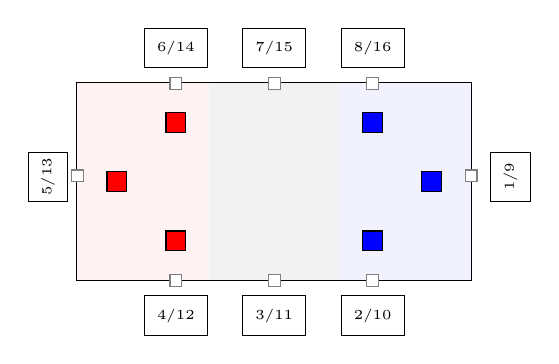
\begin{tikzpicture}[scale=0.25] % größere Darstellung
% Maße (m)
\def\L{20}   % Länge (x)
\def\W{10}   % Breite (y)

% Rahmen
\draw[thick] (0,0) rectangle (\L,\W);

% Sektionen entlang der x-Achse (3 gleich große à ~8.33 m)
% Farbig: Grenze rot|grau = rot, Grenze grau|blau = blau
\draw[dashed,red!70] (6.66,0) -- (6.66,\W);
\draw[dashed,blue!70] (13.33,0) -- (13.33,\W);

\draw[dashed,gray!70] (0,0.5) -- (\L,0.5);

% Farbige Zonen: 3 gleich große Bereiche (links rot, Mitte grau, rechts blau)
\fill[red!5]   (0,0) rectangle (6.66,\W);
\fill[gray!10] (6.66,0) rectangle (13.33,\W);
\fill[blue!5]  (13.33,0) rectangle (\L,\W);

% Rand-Boxen an allen Maß-Enden (außen liegend)
% oben und unten an x = 5,10,15 (Ecken ausgenommen)
\foreach \x in {5,10,15}{
\draw[draw=gray,fill=white] (\x-0.3,-0.3) rectangle ++(0.6,0.6);      % unten, außen
\draw[draw=gray,fill=white] (\x-0.3,\W-0.3) rectangle ++(0.6,0.6); % oben, außen
}
% links und rechts an y = 3.33,6.66 (Ecken ausgenommen)
\draw[draw=gray,fill=white] (-0.3,5.0) rectangle ++(0.6,0.6);       % links, außen
\draw[draw=gray,fill=white] (\L-0.3,5.0) rectangle ++(0.6,0.6); % rechts, außen


% Beispiel-Targets (weiße Quadrate)
% Linke drei Boxen rot
\foreach \x/\y in {5/2, 2/5, 5/8}{
\draw[fill=red] (\x-0.5,\y-0.5) rectangle ++(1,1);
}
% Rechte drei Boxen blau (alle im blauen Segment > 16.66)
\foreach \x/\y in {15/2, 18/5, 15/8}{
\draw[fill=blue] (\x-0.5,\y-0.5) rectangle ++(1,1);
}

	% ArUco Marker außerhalb des Feldes (größer und weiter außen)
	% Top side: Markers 18/17, 20/19, 22/21, 24/23
    \draw[fill=white,draw=black] (5-1.6,\W+0.8) rectangle ++(3.2,2.0);
	\node[font=\tiny] at (5,\W+1.8) {6{/}14};
	\draw[fill=white,draw=black] (10-1.6,\W+0.8) rectangle ++(3.2,2.0);
	\node[font=\tiny] at (10,\W+1.8) {7{/}15};
	\draw[fill=white,draw=black] (15-1.6,\W+0.8) rectangle ++(3.2,2.0);
	\node[font=\tiny] at (15,\W+1.8) {8{/}16};

	% Bottom side: Markers 12/11, 10/9, 8/7, 6/5
	\draw[fill=white,draw=black] (5-1.6,-2.8) rectangle ++(3.2,2.0);
	\node[font=\tiny] at (5,-1.8) {4{/}12};
	\draw[fill=white,draw=black] (10-1.6,-2.8) rectangle ++(3.2,2.0);
	\node[font=\tiny] at (10,-1.8) {3{/}11};
	\draw[fill=white,draw=black] (15-1.6,-2.8) rectangle ++(3.2,2.0);
	\node[font=\tiny] at (15,-1.8) {2{/}10};

	% Left side: Markers 16/15 (oben), 14/13 (unten)
	\draw[fill=white,draw=black] (-2.5,5.0-1.0) rectangle ++(2.0,2.5);
	\node[font=\tiny,rotate=90] at (-1.5,5.0+0.25) {5{/}13};

	% Right side: Markers 2/1 (oben), 4/3 (unten) - weiter nach rechts
	\draw[fill=white,draw=black] (\L+1.0,5.0-1.0) rectangle ++(2.0,2.5);
	\node[font=\tiny,rotate=90] at (\L+2.0,5.0+0.25) {1{/}9};

\end{tikzpicture}
\caption{ArUco Marker ID's}
\label{fig:aruco-markers}
\end{figure}
The ArUco markers are from the $DICT\_4\times4\_50$ dictionary and have a size of 0.5m x 0.5m. This information enables positioning in the arena with a view of a single marker.

\subsection[Arbiter / Judge]{\textcolor{blue}{Arbiter / Judge}}
\begin{itemize}
	\item{A Ground Truth and Scoring Display visible to both teams is desired. This display should show the current match scores.}
	\item{However, no technical solution is provided by the organizers that collects or distributes real-time information on positioning, scoring, or any other referee-related data.}
	\item{Teams are therefore encouraged to develop their own sensing and evaluation systems if they wish to monitor swarm position or performance metrics during the match.}
\end{itemize}
\color{black}
